\chapter{Implementación}
     En este capítulo se explican los detalles de la implementación de las partes FrontEnd y BackEnd de nuestro proyecto, tanto de la generación del proyecto inicial como de la infraestructura del mismo.
    
    
    \section{FrontEnd}
    En esta sección se va a hablar del proyecto Angular el cual compone la parte FrontEnd de nuestra aplicación. Este framework nos ofrece un desarrollo más rápido con respecto a otros frameworks, ya que se estructura en diferentes componentes web y genera una página web dinámicamente.
    \subsection{Generación Proyecto Angular}
    Para la generación de un proyecto base en Angular se utilizó \textit{Angular Cli}, un herramienta de línea de comandos que facilita la creación y gestión de proyectos Angular y de sus diferentes componentes.
    \newline
    
    \textit{Angular Cli}, al tratarse de  una herramienta NodeJS, requiere tenerlo instalado en nuestro sistema operativo. Para ello la primera tarea a realizar es instalar NodeJS a través de su página oficial\cite{nodejs}, escogiendo la versión que soporte nuestro sistema operativo.
 
    A continuación, a través del terminal que nos proporciona la herramienta de desarrollo \textit{Visual Studio Code}, ejecutamos el comando \texttt{npm install -g @angular/cli@latest}, el cual nos instala \textit{Angular Cli} en la última versión disponible.
    
    \begin{figure}[h]
    \centering
     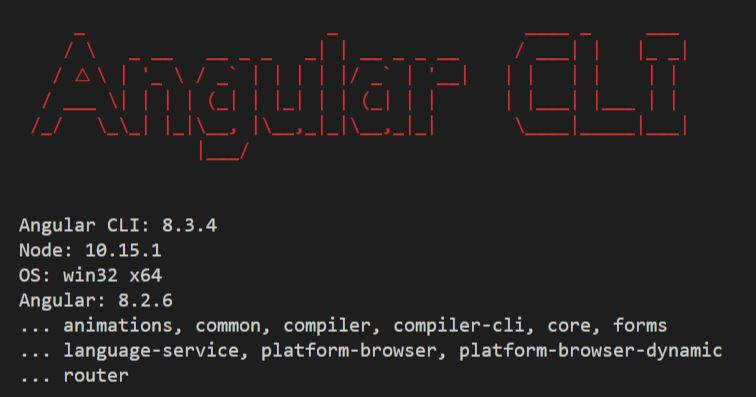
\includegraphics[width=0.65\textwidth]{images/angularversion}
    \caption{Versión Angular Cli}
    \end{figure}
    
    \FloatBarrier
    
    Una vez instalada la herramienta de comandos \textit{Angular Cli}, procedemos a crear nuestro proyecto base Angular ejecutando el comando \texttt{ng new estudio-medico-tfg2019}, generando un proyecto completo Angular junto con toda su estructura de carpetas.
    
    
    
    \subsection{Arquitectura de la aplicación Angular}
    
    \subsection{Inicialización del proyecto}
        \subsubsection{\underline{Local}}
        \subsubsection{\underline{Remoto}}
    
    
    \section{BackEnd}
    
     En esta sección se va a hablar del proyecto Java Spring Boot el cual compone la parte BackEnd de nuestra aplicación. La aplicación es una API-REST, la cual será consumida por el FrontEnd mediente llamadas en protocolo HTTP. 
     
     
    \subsection{Generación Proyecto Java Spring Boot}
    Para la generación del proyecto inicial se utilizó Spring Initializr\cite{springinitializr}, a través de su página web. Escogimos gestionar las dependencias del proyecto con Maven dado el alto grado de familiaridad que poseemos con esta tecnología. A continuación se escogió el lenguaje Java para implementar la aplicación debido a sus características intrínsecas(polimorfismo y herencia). Para finalizar se añadieron los paquetes de Web y JPA, necesarios para gestionar las conexiones externas y para la capa de persistencia.
    
    \begin{figure}[h]
    \centering
     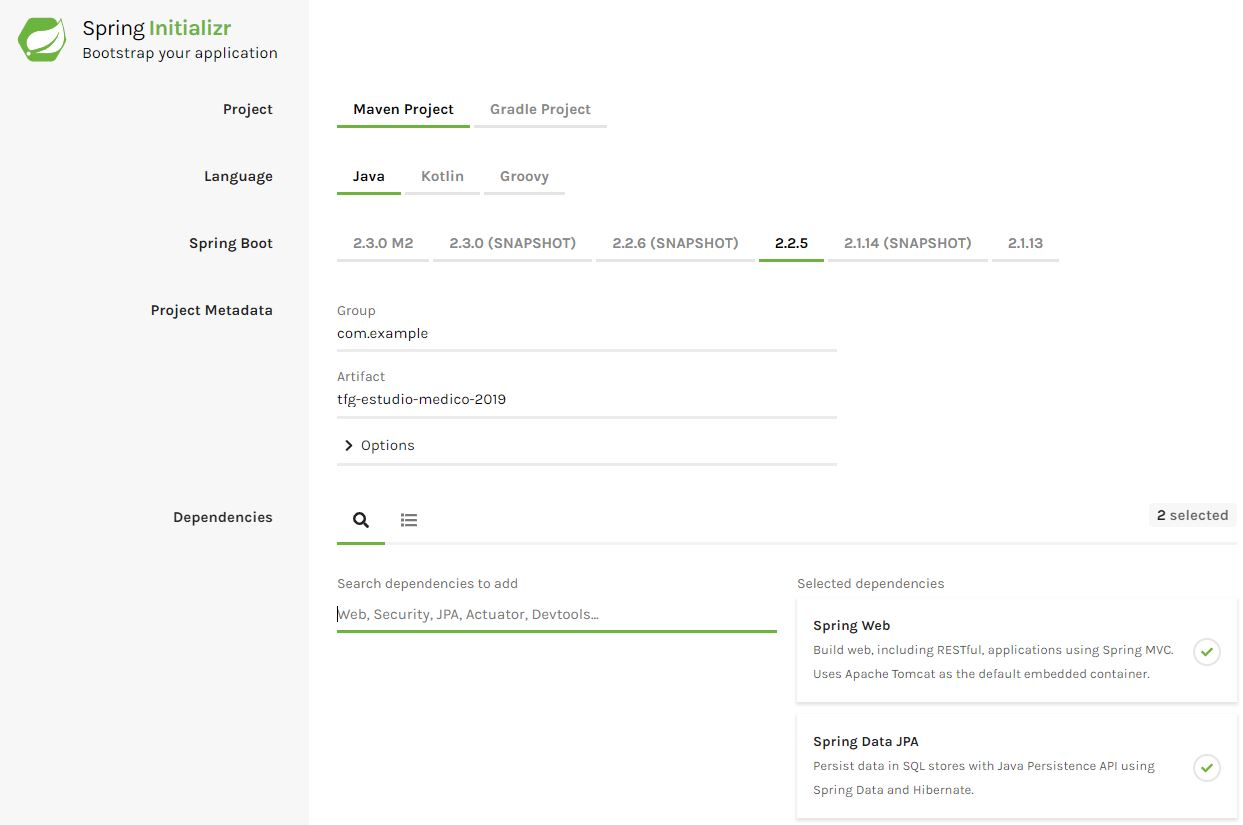
\includegraphics[width=1\textwidth]{images/springstarter}
    \caption{Proyecto inicial Spring Boot}
    \end{figure}
    
    Una vez generado el proyecto Sprinig Boot, hubo de importarse el mismo en el entorno de desarrollo Eclipse.
    
    
    \subsection{Arquitectura de la aplicación Java Spring Boot}
    La arquitectura de la aplicación Spring Boot desarrollada se divide principalmente en los apartados de código, documentación y tests.

        \subsubsection{\underline{Código}}
        El proyecto BackEnd de la aplicación está escrito en Java 8, y dividido en los siguientes bloques o paquetes, los cuales se describen a continuación.
        
        \begin{itemize}
            \item\textbf{Controladores}  \\
            Son los elementos del código encargados de recibir las diferentes peticiones HTTP y mapear los objetos enviados en las mismas, ya sea en el cuerpo de la petición en caso de ser una petición de tipo POST, o en la propia url si es una petición de tipo GET. Además de esto, son los encargados de realizar la lógica de navegación, llamando a la capa de Negocio y, con el resultado obtenido, generar una respuesta a la parte FrontEnd de la aplicación.
            \newline
            
            Para identificar los diferentes controladores de nuestra aplicación, la nomenclatura de los mismos siempre terminará con la palabra \textit{Controller}.
            \newline
            
            En nuestra aplicación disponemos de 3 controladores: El \textit{UserController}, encargado principalmente del proceso de login de la aplicación. El \textit{AdminController}, encargado de obtener todos los recursos que demande el usuario de tipo administrador en nuestra aplicación. Finalmente el \textit{ResearcherController}, encargado de obtener los recursos que demanden los usuarios de tipo investigador en nuestra aplicación.
            \newline
            
            Todos los controladores se han implementado con el patrón de Diseño \textit{Interface}, separando los métodos de su implementación y haciendo al código más legible y mantenible de cara al futuro.
            \newline
            
                \begin{figure}[h]
                    \centering
                     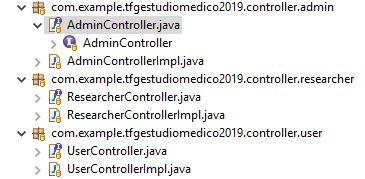
\includegraphics[width=0.8\textwidth]{images/controllers.JPG}
                    \caption{Controladores del proyecto BackEnd}
                \end{figure}
                
                \begin{figure}[h]
                \centering
                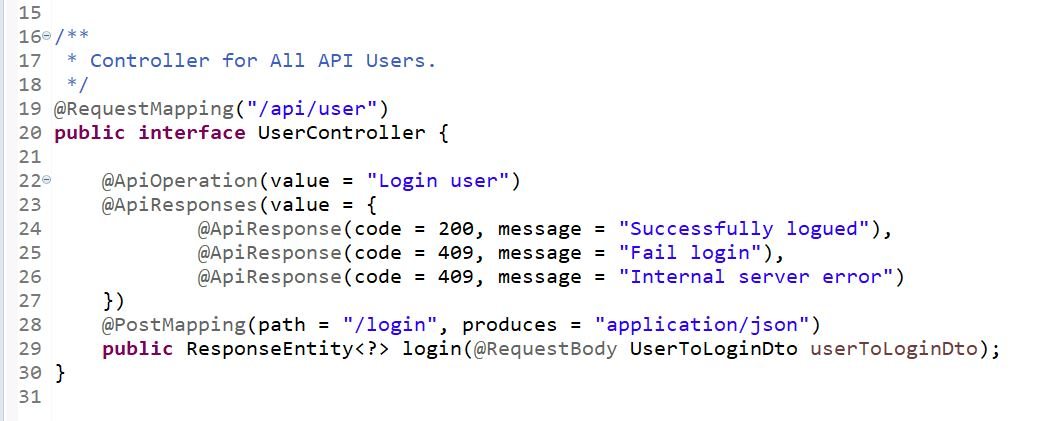
\includegraphics[width=1\textwidth]{images/usercontroller.JPG}
                \caption{Ejemplo Interfaz Controlador UserController}
                \end{figure}
                
                \FloatBarrier
            
             \item\textbf{Servicios de la aplicación}  \\
            Son los elementos del código encargados de centralizar la lógica principal de la aplicación. Los controladores los llaman, estos llaman a los repositorios para obtener los recursos solicitados, y devuelven dichos recursos al controlador.
            \newline
            
            Para identificar los diferentes servicios de de nuestra aplicación, la nomenclatura de los mismos siempre terminará con la palabra \textit{Business}.
            \newline
            
            En nuestra aplicación disponemos de 3 servicios de aplicación: El \textit{UserBusiness}, encargado principalmente de gestionar a los diferentes usuarios de la aplicación. El \textit{ResearcherBusiness}, encargado de gestionar las diferentes funcionalidades que puede realizar un usuario de tipo investigador en nuestra aplicación. Por último el \textit{SubjectBusiness}, encargado de gestionar a los pacientes y a sus respectivas citas y cuestionarios.
            \newline
            
            Al igual que los controladores, todos los servicios de aplicación se han implementado con el patrón de diseño \textit{Interface}
            \newline.
            
             \begin{figure}[h]
                \centering
                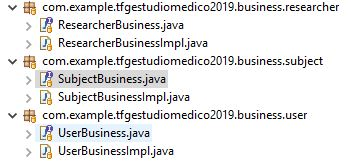
\includegraphics[width=0.8\textwidth]{images/business.JPG}
                \caption{Servicios de Aplicación del proyecto BackEnd}
            \end{figure}
            
            \begin{figure}[h]
                \centering
                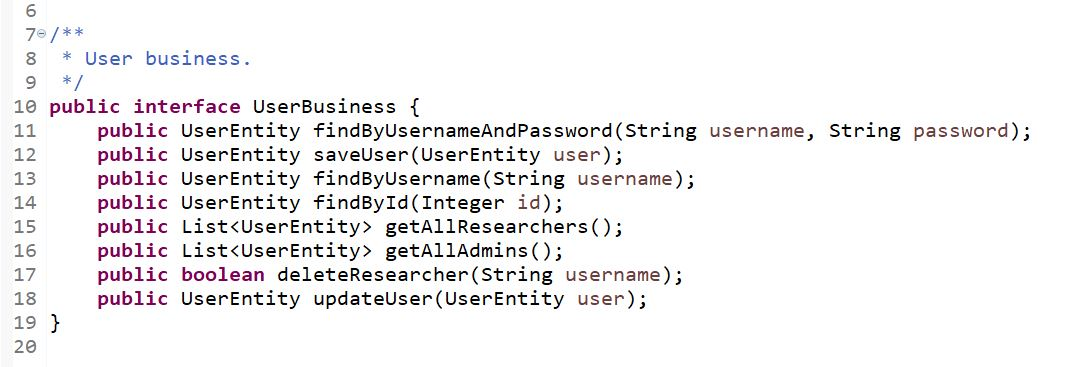
\includegraphics[width=1\textwidth]{images/userbusiness.JPG}
                \caption{Ejemplo Interfaz Servicio de aplicación UserBusiness}
            \end{figure}
            
            \FloatBarrier
            
            \item\textbf{Repositorios}  \\
            Son los elementos encargados de comunicarse con la base de datos correspodiente, ya sea guardando recursos, actualizar, listar, borrar etc... \\
            \newline
            Todos los repositorios extienden de la clase \textit{JpaRepository}, una clase perteneciente a SpringData, la cual implementa el código necesario para realizar una query a la base de datos. De esta manera no ha sido necesario implementar dichas clases.
            \newline 
            
            Para identificar los diferentes repositorios de de nuestra aplicación, la nomenclatura de los mismos siempre terminará con la palabra \textit{Repository}.
            \newline
            
            Nuestra aplicación dispone de 4 repositorios: El \textit{InvestigationDetailsRepository}, encargado de gestionar los detalles de los cuestionarios realizados a los pacientes. El \textit{InvestigationRepository}, encargado de gestionar los cuestionarios realizados a los pacientes. El \textit{UserRepository}, encargado de gestionar a los diferentes usuarios administradores e investigadores de la aplicación. Y finalmente, el
            \textit{SubjectRepository}, encargado de gestionar a los pacientes del estudio.
            \newline
            
            \begin{figure}[h]
                \centering
                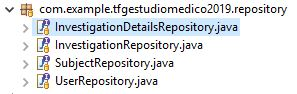
\includegraphics[width=0.8\textwidth]{images/repository.JPG}
                \caption{Repositorios del proyecto BackEnd}
            \end{figure}
            
            \begin{figure}[h]
                \centering
                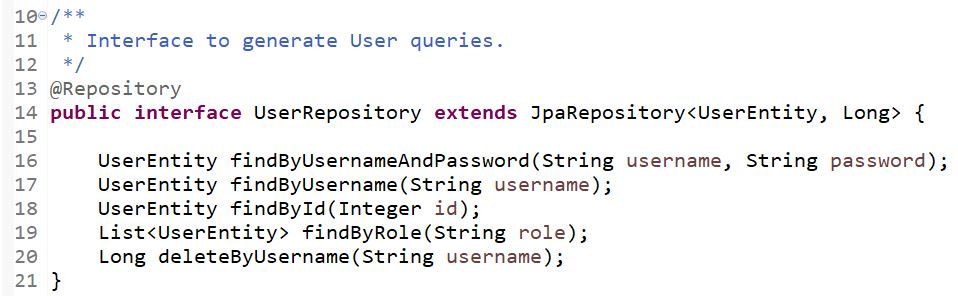
\includegraphics[width=1\textwidth]{images/userrepository.JPG}
                \caption{Interfaz Repositorio UserRepository}
            \end{figure}
            
            \FloatBarrier
            
            \item\textbf{Modelos}  \\
            Son los elementos encargados de almacenar la información de las bases de datos y de las peticiones HTTP, delimitando el dominio de las mismas.
            \newline
            
            Hay 3 tipos de modelos en nuestra aplicación:
            \begin{itemize}
                \item Dominio. \\
                Son los elementos que definen un rango de posibles valores. En nuestra aplicación disponemos del enumerado  \textit{Role} para definir los tipos de usuarios que pueden acceder a la aplicación.
                \newline
                
                 \begin{figure}[h]
                \centering
                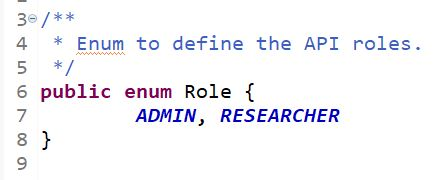
\includegraphics[width=0.9\textwidth]{images/role.JPG}
                \caption{Ejemplo Dominio Enumerado Role}
                \end{figure}
                
              
                \item Entidades.  \\
                Son los elementos encargados de interactuar con las bases de datos de nuestra aplicación. Estas entidades JPA, también llamadas POJO's(Plain Old Java Objects), se encuentran mapeadas mediante anotaciones y representan las tablas de nuestra base de datos relacional.
                \newline
                
                
            Para identificar las diferentes entidades de nuestra aplicación, la nomenclatura de las mismas siempre terminará con la palabra \textit{Entity}.
            \newline
                
                  \begin{figure}[h]
                        \centering
                        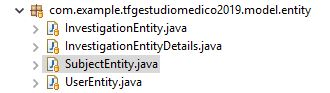
\includegraphics[width=0.8\textwidth]{images/entity.JPG}
                        \caption{Entidades del proyecto BackEnd}
                    \end{figure}
            
                    \begin{figure}[h]
                        \centering
                        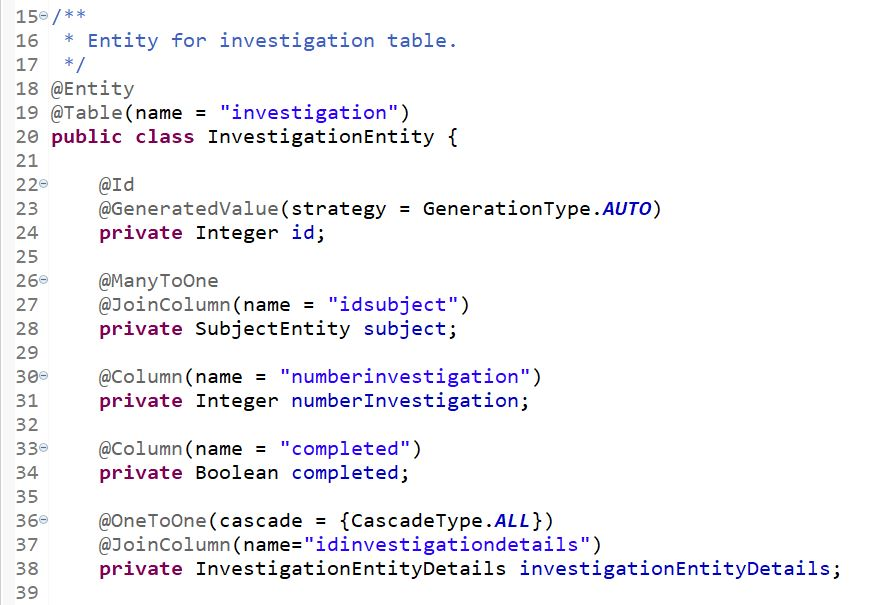
\includegraphics[width=1\textwidth]{images/investigationentity.JPG}
                        \caption{Ejemplo Entidad InvestigationEntity}
                    \end{figure}
            
            \FloatBarrier
                
                
                \item Dtos(Data Transfer Objects). \\
                Son los elementos encargados de mapear los objetos de tipo JSON enviados en las peticiones HTTP para ser tratados en la aplicación. También se encargan de devolver la información necesaria mediante una respuesta HTTP.
                \newline
                
                 Para identificar a los dtos(Data Transfer Objects) de nuestra aplicación, la nomenclatura de los misms siempre terminará con la palabra \textit{Dto}.
                \newline
                
                De esta manera, los controladores de la aplicación tratarán los dtos y los mapearán a entidades para ser tratadas en la capa de Negocio, proporcionando seguridad y robustez a la aplicación, evitando posibles inyecciones de código y protegiendo los campos sensibles que no deban mostrarse en el exterior.
                \newline 
                
                    \begin{figure}[h]
                        \centering
                        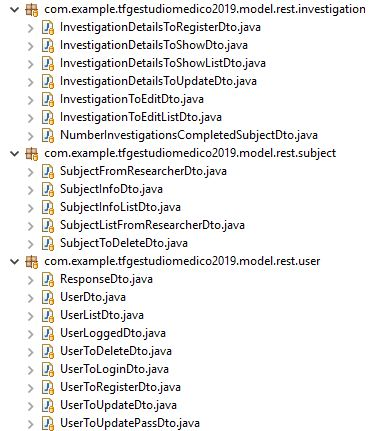
\includegraphics[width=0.8\textwidth]{images/dto.JPG}
                        \caption{Dtos del proyecto BackEnd}
                    \end{figure}
            
                    \begin{figure}[h]
                        \centering
                        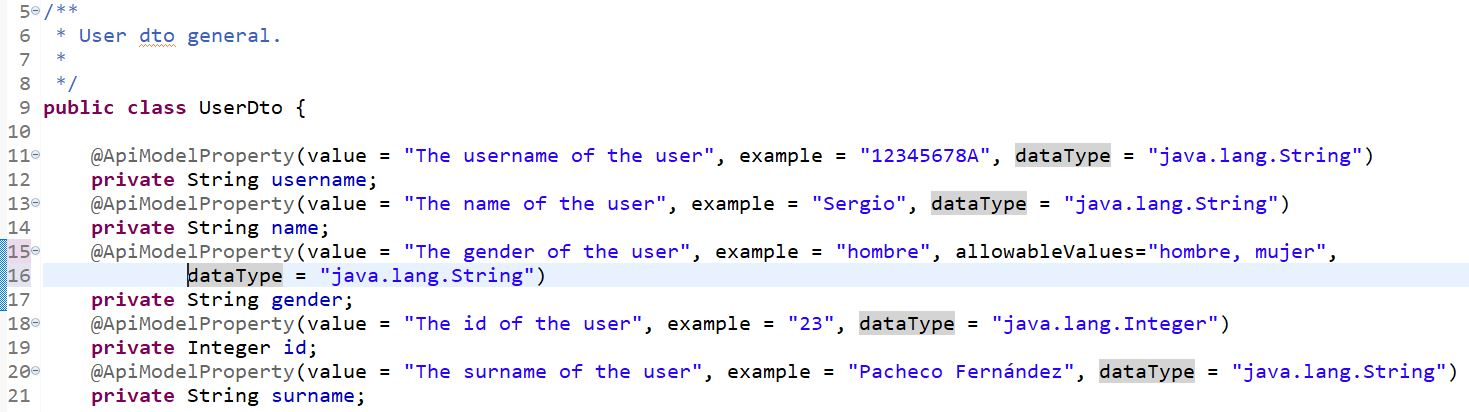
\includegraphics[width=1\textwidth]{images/userdto.JPG}
                        \caption{Ejemplo dto UserDto}
                    \end{figure}
            
            \FloatBarrier
                
                
            \end{itemize}
            
            
        \end{itemize}
        \subsubsection{\underline{Documentación}}
        A la hora de documentar la aplicación BackEnd, por una parte, se utilizó \textit{Javadoc} al principio de cada clase Java, y por otro lado, se utilizó \textit{Swagger}. 
        \newline
        
        Para utilizar el framework \textit{Swagger} en la aplicación, hubo de añadir las correspondientes dependencias en el archivo \textit{pom.xml}.
        \newline
        
        \begin{figure}[h]
            \centering
            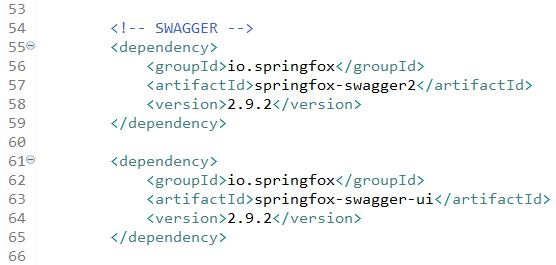
\includegraphics[width=1\textwidth]{images/swagger.JPG}
            \caption{Dependencias Swagger añadidas en pom.xml}
        \end{figure}
        
        \textit{Swagger} nos permitió documentar tanto los endpoints como los dtos de nuestra aplicación a través de anotaciones, las cuales se añadieron en las respectivas clases implicadas.
        
          \begin{figure}[h]
            \centering
            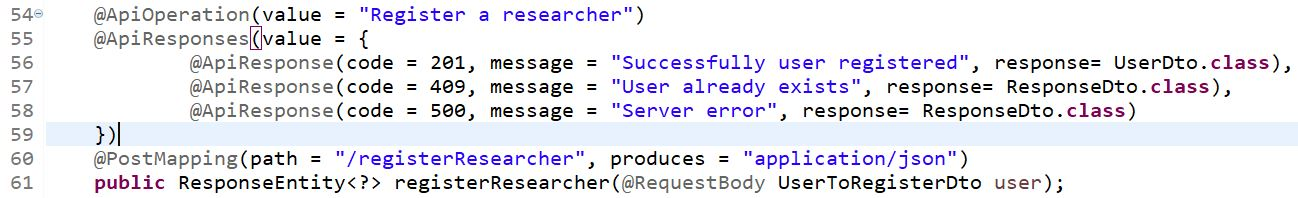
\includegraphics[width=1\textwidth]{images/swaggerexample.JPG}
            \caption{Ejemplo Documentación Swagger en el endpoint Registrar Investigador}
        \end{figure}
        
        
         \textit{Swagger} posee una interfaz llamada swagger.ui a la cual se puede acceder una vez arrancado el proyecto BakEnd para realizar pruebas y comprobar la documentación generada, como se muestra continuación. Dicha interfaz documenta tanto la información general de la aplicación, como los endpoints y los dtos.
         \newline
         
          \begin{figure}[h]
            \centering
            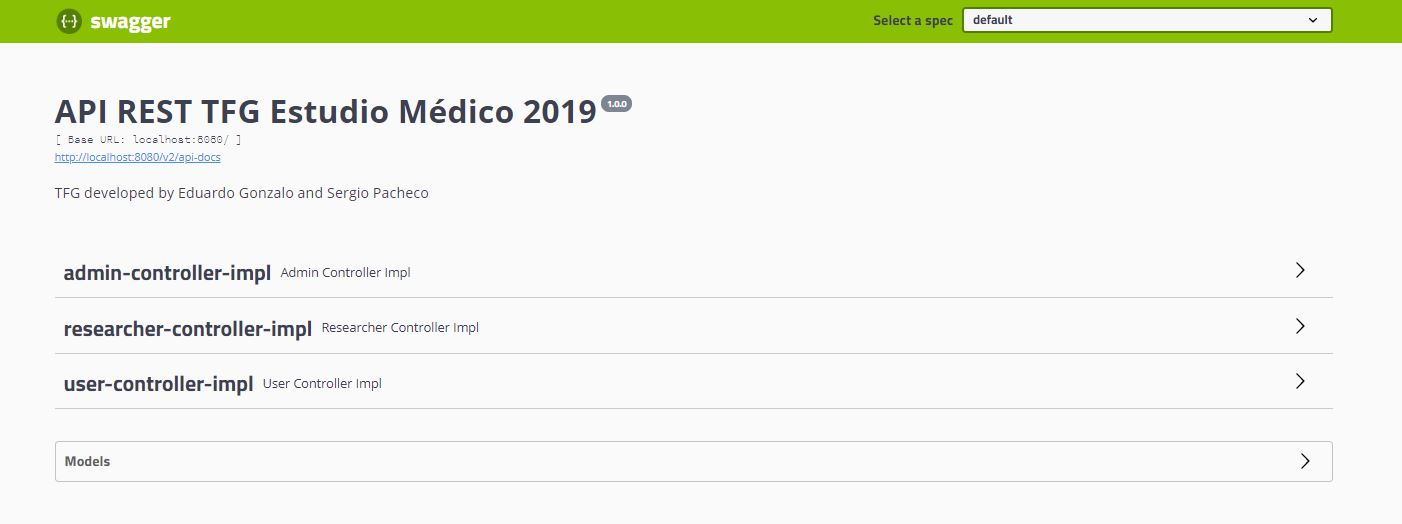
\includegraphics[width=1\textwidth]{images/swaggergeneral.JPG}
            \caption{Interfaz swagger.ui}
        \end{figure}
        
          \begin{figure}[h]
            \centering
            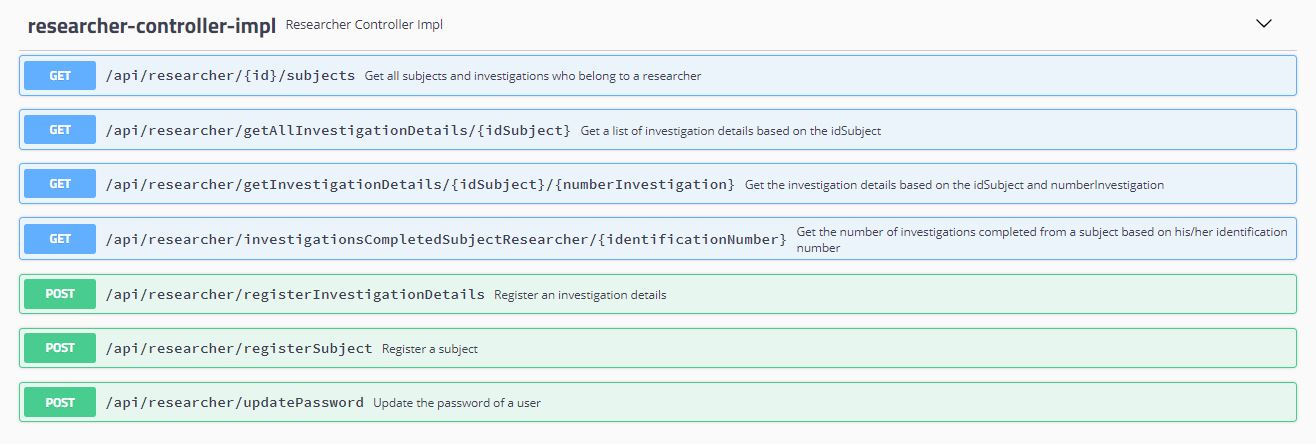
\includegraphics[width=1\textwidth]{images/swaggerendpoint.JPG}
            \caption{Ejemplo Documentación Swagger Researcher Controller}
        \end{figure}
        
        \begin{figure}[h]
            \centering
            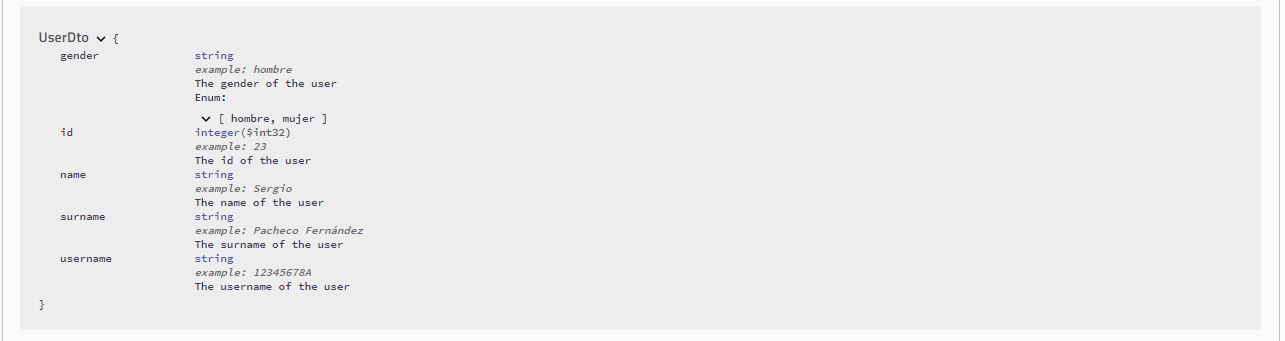
\includegraphics[width=1\textwidth]{images/swaggeruserdto.JPG}
            \caption{Ejemplo Documentación Swagger UserDto}
        \end{figure}
        
        \FloatBarrier
        
        
        \subsubsection{\underline{Tests}}
        A la hora de garantizar la calidad del software, se han realizado tests con Mockito y JUnit. Se han testeado todos los métodos de todas las clase que poseen lógica(Controladores y Servicios de Aplicación), probando todos los caminos y excepciones posibles, así como el camino feliz.
        \newline
        
        En la aplicación hay un total de 157 tests realizados, los cuales se ejecutan cada vez que se instala la aplicación, garantizando así el correcto funcionamiento de la misma.
        \newline
        
          \begin{figure}[h]
            \centering
            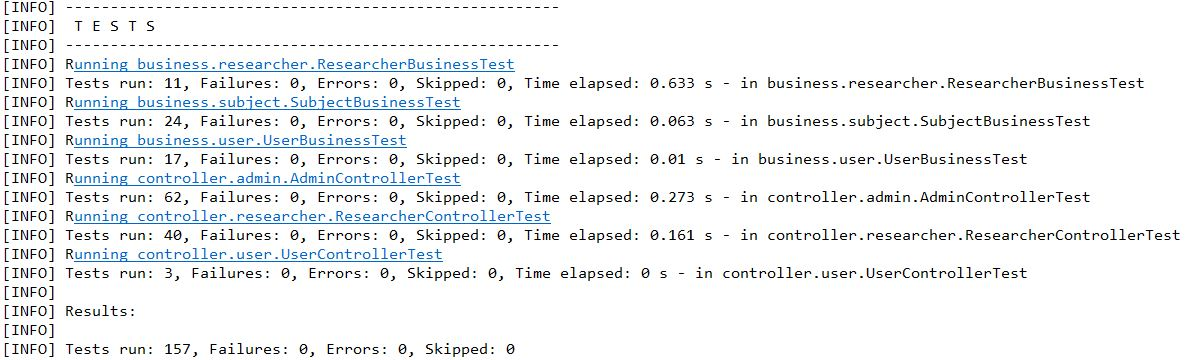
\includegraphics[width=1\textwidth]{images/numtests.JPG}
            \caption{Tests realizados en la aplicación}
        \end{figure}
        
        Para garantizar que se han testeado todos los caminos posibles, se ha conseguido un 100\% de cobertura en todas las clases con tests.
        \newline
        
        
          \begin{figure}[h]
            \centering
            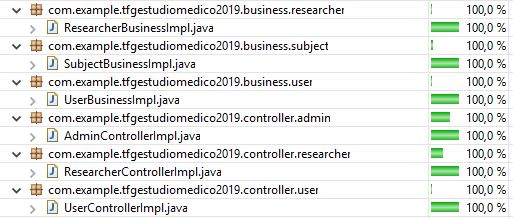
\includegraphics[width=1\textwidth]{images/coberturatests.JPG}
            \caption{Cobertura de las clases testeadas}
        \end{figure}
        

        
        
    \subsection{Inicialización del proyecto}
        A la hora de inicializar la aplicación BackEnd, al tratarse de un proyecto  Maven, lo primero que hay que ejecutar son los siguientes comandos: 
        
        \begin{enumerate}
          \item\texttt{mvn clean}.\\
          Elimina los archivos generados anteriormente y descarga las librerías añadidas como dependencias en el archivo pom.xml
          \item\texttt{mvn install}. \\
          Genera el archivo .jar definido en el pom.xml
        \end{enumerate}
        
        Si queremos ejecutar la aplicación BakEnd de manera local, lo único que tenemos que hacer es ejecutar la clase \texttt{Main} de la aplicación en el entorno de desarrollo elegido, en este caso, Eclipse. \\
        \newline
        Si queremos ejecutar la aplicación BakEnd de manera remota, solo tenemos que almacenar el archivo .jar generado anteriormente en el servicio de Hosting escogido, en este caso, en Hostinger\cite{hostinger}.
        
        
        
        
    